\chapter{Fyzikální model}

\section{Model kamene}
Broušený kámen je modelován jako konvexní mnohostěn \cite{Pohl2002}. Brusné kotouče považujeme za dokonale rovinné. Uchycení kamene při broušení zjednodušíme na absolutně tuhé bez známek pružnosti či ohybu. Fasety potom můžeme modelovat jako rovné plochy. Orientace a umístění fasety získáme z výkresu nebo předchozího měření. 

Přechody mezi fasetami jsou v ideálním případě ostré hrany. Z důvodu abraze hran v procesu výroby kamene jsou hrany obroušeny do oblého tvaru. K přiblížení modelu reálnému obroušení hran aproximujeme hranu množstvím rovinných faset se vzájemnou polohou odpovídající poloměru křivosti hrany.  
  
\begin{figure}[htps]
\centering
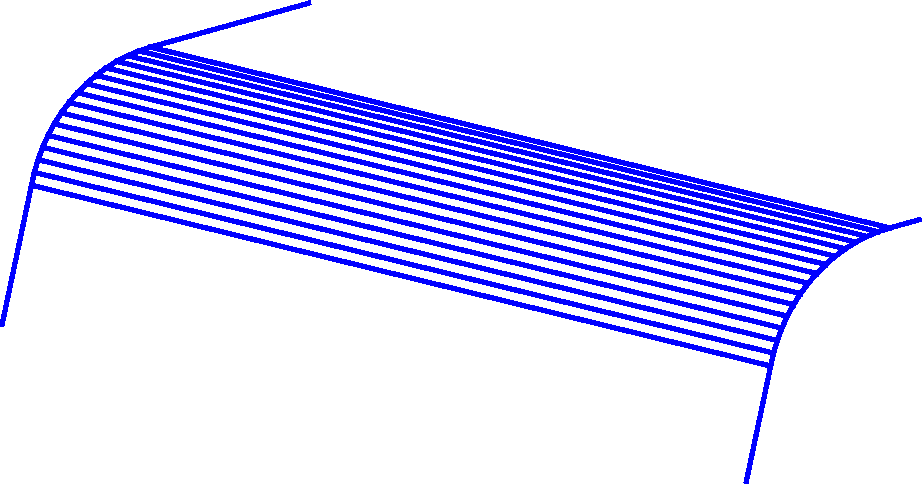
\includegraphics[width=0.6\linewidth]{edge_ex.pdf}
\caption{Detail aproximace přechodu mezi fasetami.}
\label{fig: edge}
\end{figure}  

\section{Model svazku}
Svazek světla v LADOKU reprezentuje nerozbíhající se konvexní hranol. Vlivem odrazu a lomu se konvexní tvar zachová. Fasety jsou také konvexní, proto se konvexita zachová i při štěpení svazku. Po opuštění kamene jsou svazky definovány zářivým tokem, plochou a směrem, které lze vyjádřit pomocí azimutu a elevace. Stokesovy koeficienty definují elektromagnetické vlastnosti svazku. 

Zaznamenána je celá cesta svazku. V každém bodě trasy máme k dispozici posloupnost směrů a tvarů svazku vyjádřeném pomocí polygonu. 

Model nepostihuje situace, při kterých nastává rozbíhavost světla.
\begin{itemize}
\item Pokud jsou v materiálu přítomné nečistoty, praskliny, vzduchové bubliny apod., světelný svazek se rozptýlí.
\item  Rozptyl světelných svazků vzniká vlivem nedokonalého vyleštění faset a to jak při lomu tak při odrazu.
\item Vlivem oxidace při leštění mohou vzniknout místa s jiným indexem lomu než je index lomu materiálu. Podobný případ nastane pokud má kámen nejednotný odstín.

\item Přítomnost hran v kameni způsobí ohyb světla (difrakci).
\end{itemize}

Část zářivého toku svazku může být pohlcena a přeměněna na teplo.

\section{Model stínítka}
\label{sec:stinitko}
Po dopadu laserového svazku na stínítko se záření difuzně odrazí. Odrazivé vlastnosti materiálu závisí na úhlu odpadajícího světla a lze je matematicky popsat pomocí modelu zvaného BRDF (Bidirectional reflectance distribution function). Odražené světlo zvýší intenzitu světla nejen v místě dopadu světelného svazku, ale i v jeho okolí.

Odražené světlo zároveň putuje do kamene a od něj zpět na stínítko. 

%%tohle bych zařadil na později
%Laserové stopy chceme detekovat v černobílém HDR snímku půlkulového stínítka, na které dopadá část laserových svazků vystupujících z nasvíceného kamene. Snímek ze zatížen radiálním zkreslením, které je způsobeno vlastností optické soustavy objektivu. Radiální zkreslení bylo určeno v předchozí bakalářské práci \cite{Drapela}. Snímek lze pomocí transformace z \cite{Drapela} zkreslení zbavit. Z \cite{Drapela} navíc známe transformaci mezi pozicí bodu v nezkresleného snímku a odpovídajícím parametrům azimutu a elevace.



V ideálním případě lze ve snímaném obraze pozorovat pouze dopady světelných svazků, které vznikly kombinací odrazů a lomů zdrojového svazku od faset broušeného kamene. U reálného kamene ovšem v obraze pozorujeme tenké slábnoucí přímky vycházející ze stopy světelného svazku, ocásky. Tyto ocásky vznikají díky lomu/odrazu světelného svazku od neostrých hran broušeného kamene.

\begin{figure}[h!]
\begin{center}
\scalebox{.9}{ \input{xfig/tails.pstex_t}}
\end{center}
\caption{Příklad snímaného obrazu s vyznačením obrazů svazků a ocásků.}
\label{fig:tail_ex1}
\end{figure}


Vnik ocásků si ukážeme při lomu světla na oblé hraně kamene. Situaci budeme uvažovat v 2D prostoru, kde platí obecně stejné principy jako ve 3D. Světlo nahradíme paprsky světla se směrem šíření $\vec{v_i}$. 

Zvolíme si dvě fasety, které svírají úhel \SI{45}{\celsius}. Ostrý přechod aproximujeme. Vznikne posloupnost úseček, které propojují fasety. Každé úsečce přiřadíme normálový vektor $\vec{n}$.  

\begin{figure}[htp]
\centering
\begin{minipage}[c]{0.48\textwidth}
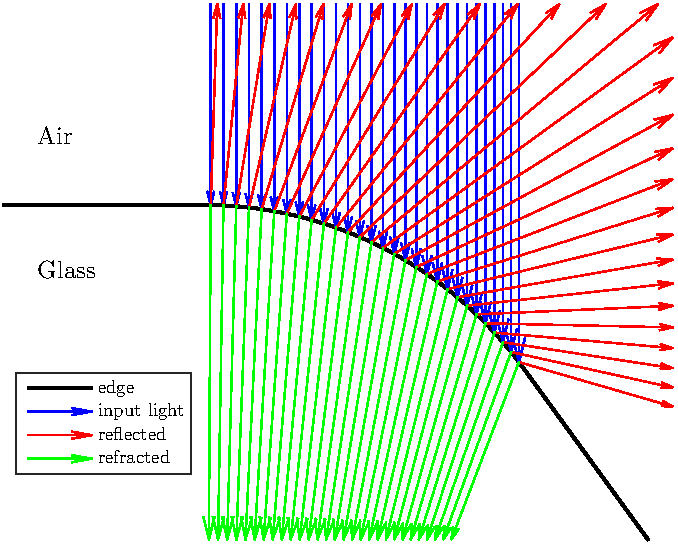
\includegraphics[width=\textwidth]{edgeIn.pdf}
\end{minipage}
\begin{minipage}[c]{0.48\textwidth}
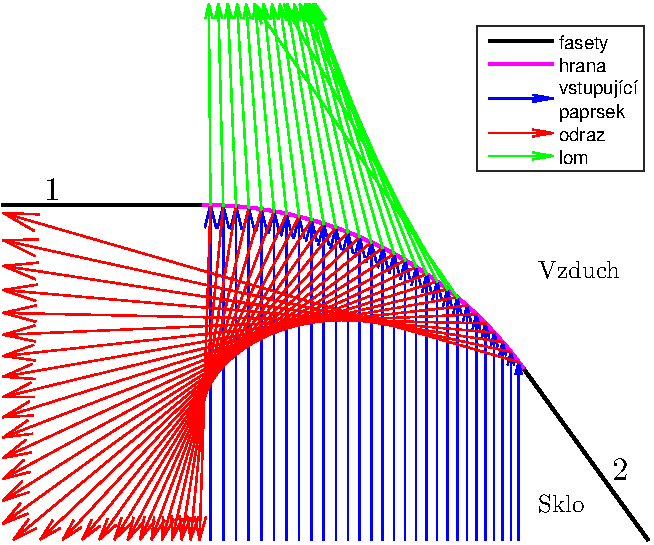
\includegraphics[width=\textwidth]{edgeOut.pdf}
\end{minipage}
\caption{Dopad světelných paprsků na hranu. Paprsky se lomí vlevo ze vzduchu do skla a vpravo ze skla do vzduchu. Situace pro index lomu vzduchu $n_a = 1$ a index lomu skla $n_g = 1.5$.}
\label{fig:edgeIn}
\end{figure}
Z Fresnelových rovnic víme, že dochází nejen k lomu světla, ale část světla000 se odrazí. Poměr intenzity odraženého a lomeného světla závisí na polarizaci světla a dopadajícím úhlu. V této ukázce uvažujeme nepolarizované světlo. 

Aplikací Snellova zákonu a zákonu odrazu na $\vec{n}$ a $\vec{v_i}$ vypočítáme směr lomu a odrazu světelných paprsků.

Na obr. \ref{fig:edgeIn} dopadají paprsky světla ze vzduchu na sklo i ze skla do vzduchu. V odou případech se odražené i lomené paprsky projeví jako ocásky.

Pokusíme se prozkoumat intenzitu ocásků $I$ v závislosti na vystupujícím úhlu, elevaci $\varepsilon$. 
Pro jednotlivou elevaci určíme intenzitu relevantně ke vstupující intenzitě jako 
\begin{equation}
 I_\varepsilon  = \frac{\rho_{{max}}}{\rho_\varepsilon}\cdot R
\end{equation}
pro odražené paprsky a 
\begin{equation}
 I_\varepsilon  = \frac{\rho_{\varepsilon_{max}}}{\rho_\varepsilon}\cdot (1-R)
\end{equation}
pro lomené paprsky, kde  

	\begin{tabular}{l l}
	$\rho_{\varepsilon}$ & 	- hustota paprsků pro danou elevaci $\varepsilon\,$,\\
	$\rho_{{max}}$  	&	- maximální hustota paprsků ve všech elevacích,\\
	$R_\varepsilon$		&	- odrazivost z Fresnelových rovnic pro $\varepsilon\,$.	 \\
	
	\end{tabular}

Závislost $I(\varepsilon)$ je označená jako \textit{Reflection coefficient} resp. \textit{Refraction coefficient} na obrázcích \ref{fig:edgeInGraf} a \ref{fig:edgeOutGraf}.


\begin{figure}[htps]
\centering
\begin{minipage}[c]{0.48\textwidth}
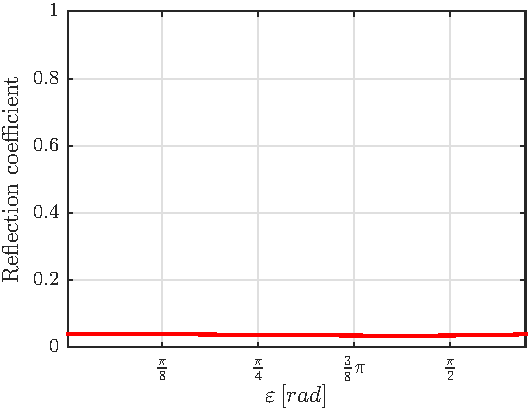
\includegraphics[width=\textwidth]{edgeIn_reflection.pdf}
\end{minipage}
\begin{minipage}[c]{0.48\textwidth}
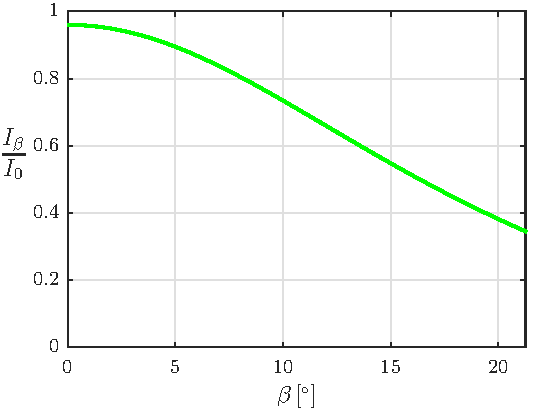
\includegraphics[width=\textwidth]{edgeIn_refraction.pdf}
\end{minipage}
\caption{\textit{Reflection coefficient} resp. \textit{Refraction coefficient} v případě když se lomí světlo ze vzduchu do skla (obr. \ref{fig:edgeIn}).}
\label{fig:edgeInGraf}
\end{figure}

\begin{figure}[htps]
\centering
\begin{minipage}[c]{0.48\textwidth}
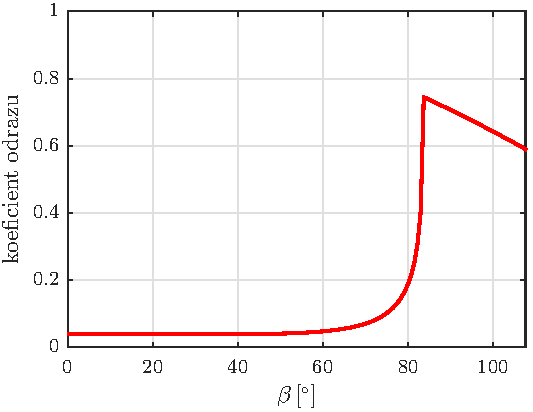
\includegraphics[width=\textwidth]{edgeOut_reflection.pdf}
\end{minipage}
\begin{minipage}[c]{0.48\textwidth}
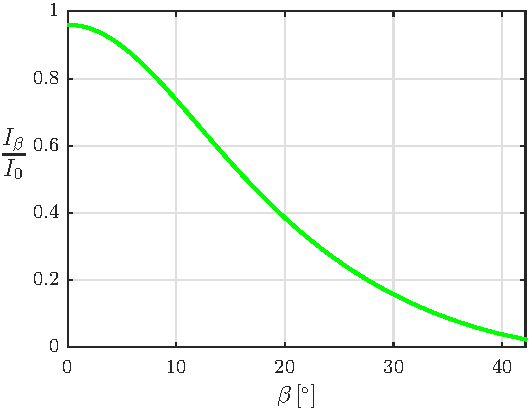
\includegraphics[width=\textwidth]{edgeOut_refraction.pdf}
\end{minipage}
\caption{\textit{Reflection coefficient} resp. \textit{Refraction coefficient} v případě když se lomí světlo ze skla do vzduchu (obr. \ref{fig:edgeIn}).}
\label{fig:edgeOutGraf}
\end{figure}

Z grafů \ref{fig:edgeInGraf} a \ref{fig:edgeOutGraf} je patrné, že ocásky budeme pozorovat různě dlouhé a z vysokou variabilitou z hlediska intenzity. 
	  

 Intenzita a délka ocásku je ovlivněna i dalšími faktory, jako je např. délka hrany, čistota hrany, drsnost povrchu atd. Všechny faktory, které ovlivňují intenzitu ocásku prozatím nejsme schopni v programu LADOK zahrnout do matematického modelu, proto pro prování svazků bude užitečná především informace o směru ocásku. 
 
 

\section{Model obrazu}

Obraz snímaný kamerou je zatížen radiálním zkreslením. Zkreslení odstraníme pomocí kalibrace kamery \cite{Drapela}. 


\section{Model Kamery}
\label{sec:poisson}
 Použitý CCD snímač má $2050^2$ pixelů. Každému pixelu odpovídá jeden samostatný snímač, který funguje na principu počítání přicházejících fotonů po dobu expozice. Počet přicházejících fotonů v daném časovém intervalu se řídí Poissonovým rozdělením. Pravděpodobnost, že napočítáme $n$ fotonů je 
 
 \begin{equation}
    P(\mathrm{X} = n)=\frac{\lambda ^{n}\,\mathrm{e}^{-\lambda}}{n!}\,,
 \end{equation}
 kde $\lambda$ je střední hodnota a $\mathrm{X}$ náhodná veličina.












